\documentclass[border=4pt]{standalone}
\usepackage{tikz}
\usetikzlibrary{arrows.meta,positioning}
\begin{document}
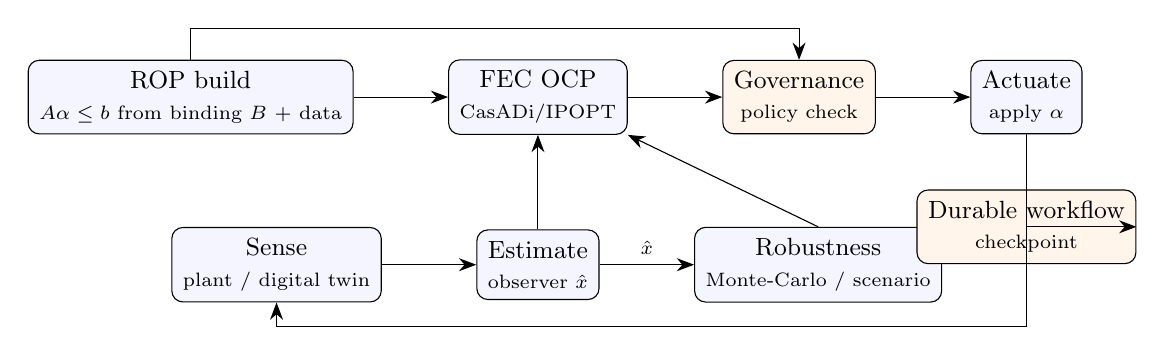
\begin{tikzpicture}[
  font=\small,
  box/.style={draw, rounded corners, align=center, minimum height=8mm, inner sep=4pt, fill=blue!4},
  gov/.style={draw, rounded corners, align=center, minimum height=8mm, inner sep=4pt, fill=orange!8},
  >={Stealth[length=2.2mm]}, node distance=7mm and 12mm]
\node[box] (rop) {ROP build\\ \scriptsize $A\alpha\le b$ from binding $B$ + data};
\node[box, right=of rop] (fec) {FEC OCP\\ \scriptsize CasADi/IPOPT};
\node[gov, right=of fec] (opa) {Governance\\ \scriptsize policy check};
\node[box, right=of opa] (act) {Actuate\\ \scriptsize apply $\alpha$};
\node[box, below=12mm of fec] (est) {Estimate\\ \scriptsize observer $\hat{x}$};
\node[box, left=of est] (sense) {Sense\\ \scriptsize plant / digital twin};
\node[box, right=of est] (mc) {Robustness\\ \scriptsize Monte-Carlo / scenario};
\node[gov, below=7mm of act, align=center] (wf) {Durable workflow\\ \scriptsize checkpoint};
\draw[->] (rop) -- (fec);
\draw[->] (fec) -- (opa);
\draw[->] (opa) -- (act);
\draw[->] (act) |- (wf.east);
\draw[->] (sense) -- (est);
\draw[->] (est) -- node[above,font=\scriptsize]{$\hat{x}$} (mc);
\draw[->] (est.north) -- (fec.south);
\draw[->] (mc.north) -- (fec.south east);
\draw[->] (act.south) |- ([yshift=-3mm]sense.south) -| (sense.south);
\draw[->] (rop.north) -- ++(0,4mm) -| (opa.north);
\end{tikzpicture}
\end{document}
